\chapter{Introduction}

\section{The Hot Big Bang model}

The most accepted model for the origin of the universe is the Big Bang model, which surprisingly to some conveys no "bang", but the sudden existence of all the matter in the universe, in the shortest of times, in the smallest of spaces, about 13.8 billion years ago. After an unthinkably small interval of time, the universe began a short period of rapid expansion known as \textit{cosmic inflation}, in which the universe grew by a factor $10^{27}$ in a mere $10^{-33}$ seconds. This inflation is thought to be due to the inflaton, a quantum scalar field theory. It is theorized that it is the inflaton's vaccuum energy what caused the universe to expand as greatly.

After this inflation phase, the universe cooled enough for what is known as the Quark-Gluon plasma to form. In this state, temperatures were high enough as to consider relativistic the random motion of the particles in it. After some cooling due to cosmic expansion, the combination between quarks to form hadrons was allowed, leading to what is known as the hadronic epoch. However, due to the short mean free path of the photons the universe is still opaque to electromagnetic radiation.

As the universe kept expanding the densities and the temperatures cooled, the existence of atoms was starting to be allowed, the $He^{+}$ and $H$ atoms. This period would finish at the universe age of $380,000$ years, moment known as recombination. Though the name `recombination' implies the fact that the universe used to be `combined' and then ceased to be so, it just comes from the fact that recombination was theorized before the Big Bang theory was thought of.

As soon as recombination ends, the excited electrons which are now orbiting neutral atoms, fall to a lower energy state, thus emmitting photons in great densities. This emmision is known as the Cosmic Microwave Background (CMB) and is the oldest direct measurement we can take of the unvierse.


\begin{figure}[h]
	\centering
	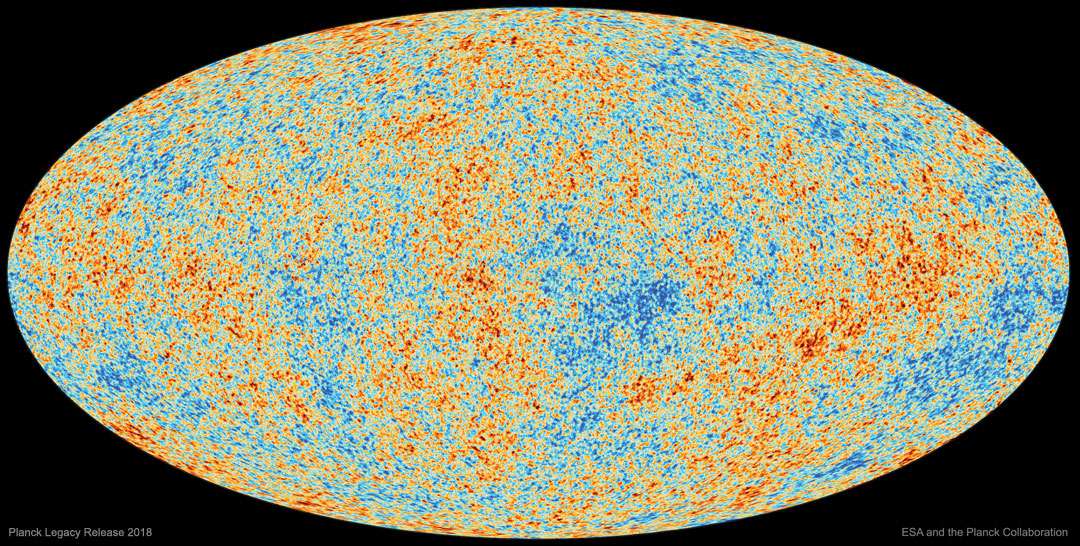
\includegraphics[width=0.8\textwidth]{../figs/cmb.jpeg}
	\caption{The CMB as seen by Space-based Observatory Planck}
	\label{fig:cmb}
\end{figure}
\section{Cosmic Microwave Background}

We see in the figure \ref{fig:cmb} the CMB as observed by the Planck colaboration \cite{Collaboration2018}. The radiaton we observe is the photons that were emmitted about $13.3$ million years ago. Since the CMB appears as a result of the thermal photons emitted by the electrons in the primordial plasma, it offers great insight into what the plasma looked like, and the way it behaved. 

As the name suggests, the CMB radiation consists of wavelengths of radiation of the order of micro meters. In fact, one can measure the associated temperature to this wavelength to be $2.7260$\SI{}{K}\cite{Fixsen2009} with some fluctuations of approximately \SI{0.0013}{K}. However, this is definitely not the temperature of the plasma before recombination. It was in fact, about $2725K$, or $\approx 1000$ times higher. This is due to the process of \textit{cosmological redshift}, which will be explained later on.

A natural question arises: How does this not break the cosmological principle? (i.e. the universe is isotropic and homogenous, meaning it is the same in every direction and at every point in space, respectively)
	
These fluctuations may be explained by the microscopic quantum oscillatios of the different fields that make up matter before and during cosmic inflation. The details of the mechanism that allows a particle to be explained as a field goes way beyond the scope of this paper, so it suffices to just mention the fact that at high enough energies, the concept of particle loses its meaning and it needs to be modeled as a constantly fluctuating field in all of space.

Thus, the CMB becomes crucial in explaining the large scale structure of the universe, since the photons that decoupled from the plasma at recombination wasted more energy leaving denser regions behind losing thermal energy in the process. 

\section{Baryon Acoustic Oscillations}

Before recombination, all matter was coupled into the same fluid which we have called the primordial plasma. The particles in the plasma interacted primarily with one another through gravity and electromagnetism, depending on the type of matter considered. 

As already mentioned, matter was not distributed homogenously so at some point in time before recombination one could find `lumps' of dark and baryonic (standard) matter. Combining the gravitational attraction between dark and baryonic matter with itself and with one another, and the repulsion caused by the Thomson Effect between baryons and photons, the results are acoustic waves propagating through the plasma, with the dark matter lumps being in the center of these waves. 

The waves would propagate throughout the plasma as long as the baryon-photon interaction was strong enough i.e. up until recombination, point in which they froze in time leaving higher density regions. Higher density means higher gravitational intensity, which means higher galaxy proliferation in spherical distributions. These spherical distributions (which can be measured in the CMB) are what is known as the large scale structure of the universe.

These structures offer a great deal  of information about the size of the `cosmic ruler' of the universe, allowing better and better accuracy in big scale cosmic measurements. The radii ($r_s \approx 150 Mpc \approx 500 $ million lightyears) of the spherical waves, the sound horizon, can be measured both in the CMB radiation, as we have already seen, and through the nearby galaxies. It has been verified that the \textit{comoving} measurements \footnote{The distance measured if the cosmological expansion did not exist} of $r_s$ is constant throughout the universe.

\section{Curvature, dark matter and the expansion of the universe}
After Hubble discovered the expansion of the universe through Hubble's Law
\begin{align}
	v = H_0 d
	\label{eq:ley-hubble}
\end{align}
With $v$ the recession speed (the speed at which some point in space is receeding only considering the expansion of the universe), $H_0=100h \frac{km}{s}Mpc ^{-1}$ Hubble's constant and $d$ the distance of said point, a great deal of studies concerning the expansion of the universe started. The most relevant result of those for this report are Friedmann's equations.
\begin{align}
	H^2(t) := \left(\frac{\dot a}{a}\right)^2 &=  \frac{8\pi G \rho}{3} +\frac{  \Lambda c^2}{3} - K \frac{c^2}{a^2}
	\label{eq:1a-friedmann}\\
	3 \frac{\ddot a}{a} &= \Lambda c^2 - 4\pi G \left( \rho + \frac{3p}{c^2} \right) 
	\label{eq:2a-friedmann}
\end{align}
In these equations we see many new paramaters. $H(t)$ is a generalization of $H_0$, $H_0$ being the value of $H(t)$ at present time. $a(t)$ is the size factor of the universe, meaning that if a certain distance measurement $\Delta x$ was taken at time $t_1$, then that same measurement would be $\frac{a(t_2)}{a(t_1)}\Delta x$ at $t_2$. $G$ is the universal gravitational constant, $\rho$ the matter density of the universe (baryonic, dark matter, etc), $\Lambda$ is the cosmological constant which contains information about Dark Energy. Finally we see $K$, which is the Gaussian Curvature of the universe. This is, asymptotical curvature.

If one managed to solve this differential equation, the result would a description of the history of the expansion of the universe. Moreover, it is also important to notice the relationship between the expansion of the universe and the distribution of matter in the universe.


Another way of writing the first Friedmann equation \eqref{eq:1a-friedmann} is by making it dimensionless 
\begin{align}
	1 = \Omega_m + \Omega_\Lambda + \Omega_k
\end{align}
Where the different $\Omega$ are defined as
\begin{align}
\Omega_m = \frac{8\pi G \rho}{3H^2}, \Omega_\Lambda = \frac{\Lambda c^2}{3H^2}, \Omega_K = -K\frac{c^2}{H^2a^2} 
\end{align}
These parameters are what define the certain cosmology we are using.

Historically, the concept of cosmological expansion appeared when Hubble observed that the radiatoion of the nearby galaxies was all shifted towards the red end of the spectrum. Of course, since the universe is expanding and the distance between two points increases with time, the wave length of a certain radiation would also be affected by this expansion. This stretching of the wave length is what is known as \textit{redshift} 
\begin{align}
	z = \frac{\lambda_{\text{o}} - \lambda_{\text{e}}}{\lambda_{\text{e}}} = \frac{\lambda_o}{\lambda_e} - 1
	\label{eq:redshift}
\end{align}
Being $\lambda_o$ the observed wavelength and $\lambda_e$ the emitted wavelength of the considered radiation. $z$ is a measure of how much the universe stretched while the radiation travelled, and it can be related to $a(t)$ through 
\begin{align}
	\frac{\lambda_o}{\lambda_e} = 1+z = \frac{a(t_o)}{a(t_e)}
\end{align}
Which means that $z$ is a temporal variable measuring the time the radiation travelled through the universe.

We thus define the comoving distance of a measurement $\Delta x$ as 
\begin{align}
	\frac{1}{1+z}\Delta x
\end{align}
i.e.\ the distance one would have measured had the expansion of the universe not existed.

With these definitions we can define  the observables we are interested in calculating/measuring. Firstly, through \eqref{eq:1a-friedmann} we calculate $H(z)$ as  
\begin{align}
	H(z) = H_0 \sqrt{\Omega_m(1+z)^3 + \Omega_k(1+z)^2 + \Omega_\Lambda} 
\end{align}
We also define the function of $z$ $D_H$
\begin{align}
	D_H(z)  = \frac{c}{H(z)}
\end{align}
Note that for $z = 0$ $D_H$ gives us an idea of the radius of the observable universe, i.e. the distance at which the recession speed is the speed of light in vacuum.

And the comoving line-of-sight distance as 
\begin{align}
	D_A = D_H\int_{0}^{z} \frac{dz}{\sqrt{\Omega_m(1+z)^3 + \Omega_k(1+z)^2 + \Omega_\Lambda} } 
\end{align}
